\documentclass[a4paper]{article}
\usepackage{lipsum}
\usepackage{url}
\usepackage{graphicx}
\usepackage{listings}
\lstset{language=Python}
\usepackage[margin=2cm]{geometry}
\usepackage{indentfirst}
\usepackage{xcolor}
\usepackage{lmodern}
\usepackage{enumitem}
\renewcommand{\familydefault}{\sfdefault}
\graphicspath{ {images/} }

\begin{document}

% TODO: Anything else needed for titlepage
\begin{titlepage}
	\newcommand{\HRule}{\rule{\linewidth}{0.5mm}}
	\center{}

    %Headings
	\LARGE{University of Nottingham}\\[1.5cm]
	\Large{Computer Science with Artificial Intelligence MSci}\\[0.5cm]
	\large{G54IRP/COMP4027 --- Individual Research Project}\\[0.5cm]

    %Title
	\HRule{}\\[0.4cm]
	{\huge\bfseries AI for General Video Game Playing}\\[0.4cm]
	\HRule{}\\[1.5cm]

    %Authors
	\begin{minipage}{0.4\textwidth}
		\begin{flushleft}
			\large
			\textit{Author}\\
			Benjamin Charlton\\
            psybc3@nottingham.ac.uk\\
            4262648
		\end{flushleft}
	\end{minipage}
    \begin{minipage}{0.4\textwidth}
		\begin{flushright}
			\large
			\textit{Supervisor}\\
			Dr.\@ Ender \"Ozcan\\
            Ender.Ozcan@nottingham.ac.uk
		\end{flushright}
	\end{minipage}

    %Date
	\vfill\vfill\vfill
	{\large7\textsuperscript{th} December 2017}
	\vfill

\end{titlepage}

%Contents Page
\pagenumbering{roman}
\tableofcontents
\pagebreak

\pagenumbering{arabic}
\section{Introduction}
\subsection{Introduction}
\begin{itemize}
    \item Popularity of Video Games
    \item Variety of Video games being played
    \item Video Games as a testing ground for AI
\end{itemize}
\subsection{Planning VS learning}
\begin{itemize}
    \item As the title says, just to get some definitions out of the way
\end{itemize}
\subsection{Motivation}
\begin{itemize}
    \item Individual desire to get better at deep reinforcement learning
    \item Learning more Methods
    \item Applying Methods
    \item Learning to use more robust and real world frameworks for DRL
    \item
    \item Seeing the state of the art in DRL and AI game playing
\end{itemize}
\subsection{Aims and Objectives}
\begin{itemize}
    \item Look at the project plan aims and objectives
\end{itemize}

\section{Related Work}
\subsection{AI and Game Playing}
\begin{itemize}
    \item AI approaches have specialised heuristics or only been developed for a single game
    \item
    \item Go --- previous interim report / PP
    \item Chess --- previous interim report / PP
    \item ALE --- Learning works for games
    \item OpenAIFive --- Learning works on big games too, and MP
    \item GET MORE THINGS FROM PP
    \item Conclusion for this section
    \item
    \item Dartmouth Workshop
\end{itemize}

\subsubsection{Early Artificial Intelligence}
%TODO: Maybe extend / re sort this section
The history of AI game playing begins near the start of artificial intelligence as a field, in the 1950s.
Strachey created a draughts player for one of the first general computing machines (Manchester Ferranti Mark I) which by  1952 could ``play a complete game of draughts at a reasonable speed''\cite{BreifHistoryComputing}.
Prinz wrote a simplified chess player for the Manchester Machine as well which could solve the mate-in-two problem.
This meant that if there was a checkmate solution in 2 turns it could successfully find it\cite{BreifHistoryComputing}.
Prinz simply used an exhaustive search technique to find the correct moves, and even though computing power was limited at the time it was clear that this wouldn't scale to full games.
This lead to Turning starting to program `Turbochamp' a chess program that would be able to play a full game of chess using heuristics\cite{BreifHistoryComputing}
\par
These simple games were made before the term artificial intelligence was being used even in an academic setting showing how natural AI and game playing go together.

\subsubsection{Deep Blue and Chess}
Chess was an early and significant example in the history of AI game playing.
In 1997 IBM managed to beat the reigning world champion, Garry Kasparov, using their custom developed machine, Deep Blue\cite{deepBlue}.
This was significant as, at the time, creating a winning chess AI was seen to be the next big milestone at the time in AI\@.
\par
To achieve this Deep Blue used a combination of techniques with the main underlying AI technique being a search method.
As Chess is a deterministic game and both players have complete information of the board state it was possible for Deep Blue to generate future board states.
With this forward model its possible to generate a search tree of possible moves and their resulting game states
The tree was efficiently generated by a combination of a massively parallel architecture over 30 nodes and the fact that each node has special purpose chess chips, generating around 6--8 moves ahead on average.
Alpha-beta pruning was used in a MinMax algorithm to help efficiently search the tree while using the custom hardware to evaluate each node quickly.
\par
IBM had proven that search methods could achieve strong results against human opponents but this was mostly due to brute force computing power and a heavy reliance on expert knowledge.
The expert knowledge came from other grandmasters and was used in the form of an opening/closing move database and the special purpose hardware to evaluate board states.
While higher computing power will always benefit AI techniques, later techniques have been developed to reduce the need of expert knowledge and to make more efficient use of hardware available.

\subsubsection{AlphaGo}
Although Deep Blue had proven that AI systems could beat an expert in games, the methods used wouldn't scale to more complex games such as Go, new methods would be needed to tackle more complex games and to further the field of AI\@.
Go was set as the next milestone in AI game playing by the community as it proved vastly more complex than chess while still having few rules and a simple goal, like chess.
To compare the difficulty between the 2 games, chess uses a 8\(\times \)8 board while Go uses a 19\(\times \)19 board.
What is a better indicator of the AI performance is the branching factor of the games for each move, as this more accurately shows how large the search tree grows for each possible move.
On average, Chess has a branching factor of 35 and Go has a branching factor of 250\cite{BranchingFactor}.
In 2016 DeepMind reached this milestone with AlphaGo claiming its victory against a 9th dan professional Go player, Lee Sedol, in March 2016\cite{alphaGo}.
\par
This achievement was accomplished with a combination of Monte Carlo Tree Search (MCTS) and 2 Deep Neural Networks trained with reinforcement learning, one was a value network to assess the board predicting the winner and the other a policy network to predict which move would be played next by an expert.
By augmenting MCTS with the policy network, the problem of the large branching factor was greatly reduced, the value network made the addition that it was quicker and more accurate at determining who would win than conventional methods and didn't require an ending game state to be reached.
Initially these networks were trained on a large number of human played games as a labeled dataset, after this `boot strapping' phase they were trained through instance of self play.
\par
Between October 2015 and AlphaGo's retirement in May 2017 there were 3 significant versions of the AI system.
AlphaGo Fan was named after its opponent Fan Hui a European 2nd dan professional Go player, where it won 5--0 being the first ever computer to beat a human professional at Go without a handicap.
AlphaGo Lee was named after its opponent Lee Sedol a South Korean 9th dan professional Go player, in this match AlphaGo won 4--1 and was seen as an AI system successfully beating a Go champion at their own game.
AlphaGo Master was the final version of the system and was named after the online account it played on for 60 Games against human opponents, it managed to win all 60 games and was finally revealed to have been a computer system to the Go community.
It finally retired at the Future of Go summit where it played a further few games beating another champion Ke Jie and a human team of 5 Go professionals.
After the summit it was clear that AlphaGo was a champion of the game and as a gift to the Go community they presented a series of 50 games for people to analyse.

\subsubsection{AlphaGo Zero}
After retiring AlphaGo Deep Mind was already working on a successor that would seek to fix some of the downsides of the AlphaGo system.
They sought to create a system that could play `tabula rasa' (latin for from a blank slate) requiring human expert decisions to learn from as they say that `Expert data sets are often expensive, unreliable or simply unavailable'\cite{alphaGoZero}.
The problem came from the initial supervised learning stage of AlphaGo's development, as it required millions of human expert games with the correct outcomes to initially learn from before it began using reinforcement learning and self play to hone its skills.
\par
There are many issues often associated with using supervised learning, 3 of the main issues were brought up when describing the expense, reliability and the availability of these datasets.
While AlphaGo had proven that there was suitable enough data for learning the game of Go, a motivating factor for the team was showing that this wasn't needed and hopefully find a method that could then later be adapted to other problems with these issues.
Another issue was a notion of a skill ceiling, as such to say that the system can only learn to be as good as the data provided to it an idea that is also seen in human learning where a student can only be as intelligent as their teachers.
This was to say that if a system learnt from human experts then it would only slightly build upon the expert knowledge where as their could potentially be ideas unconsidered by humans that could lead to a stronger system.
AlphaGo had shown evidence of this when it played a so-called `divine move' against Lee Sedol indicating there was more potential for innovation in strategy even in an ancient classic game like Go.
Furthermore by also not having a reliance on human expert knowledge an AI system could be developed to complete task where there is limited or no expert knowledge to help guide it.
\par
\begin{itemize}
    \item How did it work
    \item Achievements
\end{itemize}

\subsubsection{notes}

\begin{itemize}
    \item AlphaGo Zero
    \item AlphaZero (Chess and Shogi? too)
\end{itemize}


AlphaGo was then extended by DeepMind to create AlphaGoZero which didn't train with human data only self play\cite{alphaGoZero}.
\par
Recently AlphaGo has been beaten by a variation of itself AlphaGoZero, named as it had learnt from zero human knowledge\cite{alphaGoZero}.
AlphaGoZero learnt entirely from self-play and achieved super human performance.
This shows that not only can AI techniques successfully solve tasks but it is possible to do so with no expert knowledge.

AlphaGo Zero still had some human expert knowledge (maybe how the network was crafted to interpret the Go board)



\subsubsection{Conclusions}
\begin{itemize}
    \item Deep Blue proves that games can effectively use forward planning to beat human experts, early techniques require a lot of power so intelligent methods are needed to speed up results/improve search depth
    \item AlphaGo Fan, Lee and Master show planning is still effective but by using more advanced techniques we can generate search trees better (ANNs).
    Also shows how learning can benefit AI techniques and boost the powerful planning techniques.
    \item AlphaGo Zero shows how learning doesn't need to require expert knowledge and can just learn from lots of experience in the environment
    \item AlphaZero shows how more generic systems can still perform well allowing for techniques that could be transplanted into many environments and still perform well.
    Also showing that although dedicated hardware was used no purpose built hardware or software was used to exploit features of the games unlike previous versions or Deep Blue.
\end{itemize}


\subsection{GVGAI and VGDL}
\begin{itemize}
    \item TODO Make some notes up here
\end{itemize}
\subsection{OPEN AI GYM and GVGAI GYM}
\begin{itemize}
    \item What is OPEN AI GYM
    \item Why is OPEN AI GYM helpful for RL
    \item GVGAI GYM
    \item Initial results from GVG AI GYM paper
    \item Maybe some more here
\end{itemize}\cite{GVGAIGYM}

\subsection{Subsection to end all subsections}
\begin{itemize}
    \item Maybe something about the open AI baselines
    \item Depends what technique I would be using but I should look into that
    \item Where does reinforcement learning come into this bad buoy
\end{itemize}


\pagebreak
\section{Appendix}

\subsection{Meeting Minutes}


\pagebreak
\subsection{Work Plan}
% \begin{center}
    % 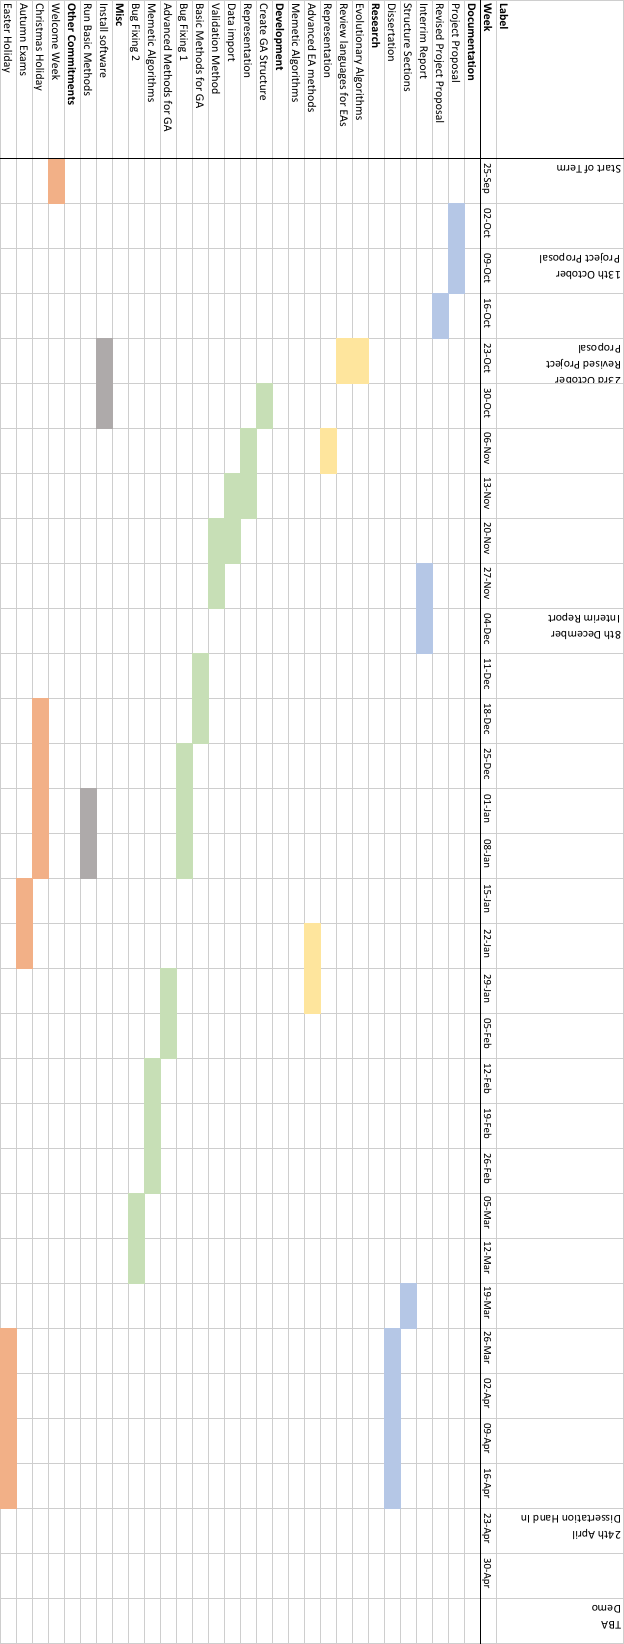
\includegraphics[height=24.8cm]{workPlan.png}
% \end{center}


%Bibliography
\subsection{References}
\bibliography{InterimReport}
\bibliographystyle{plain}


\end{document}
